\documentclass[reqno]{amsart}

\usepackage{amsfonts,latexsym,amsthm,amssymb,amsmath,amscd,euscript,bm}
\usepackage[sc]{mathpazo}
\usepackage[margin = 2.6cm]{geometry}
\usepackage{enumitem}
\usepackage{hyperref}
% sets numbering of enumerate to a, b, c, ...
\renewcommand{\theenumi}{\alph{enumi}}

% Theorems, propositions, etc.
\newtheorem{theorem}{Theorem}
\newtheorem{proposition}[theorem]{Proposition}
\newtheorem{lemma}[theorem]{Lemma}
\newtheorem{corollary}[theorem]{Corollary}

\theoremstyle{definition}
\newtheorem{definition}[theorem]{Definition}
\newtheorem*{claim}{Claim}

\theoremstyle{remark}
\newtheorem*{remark}{Remark}
\newtheorem*{notation}{Notation}

\usepackage{graphicx}



% Math blackboard font
\newcommand{\nc}{\newcommand}
\nc{\on}[1]{\operatorname{#1}}

\nc{\R}{\mathbb R}
\nc{\C}{\mathbb C}
\nc{\Q}{\mathbb Q}
\nc{\Z}{\mathbb Z}
\nc{\N}{\mathbb N}
\nc{\HH}{\mathbb H}
\nc{\DD}{\mathbb D}
\nc{\TT}{\mathbb T}
\nc{\EE}{\mathbb E}
\nc{\PP}{\mathbb P}

\nc{\cT}{\mathcal T}
\nc{\cA}{\mathcal A}
\nc{\cM}{\mathcal M}
\nc{\cR}{\mathcal R}
\nc{\cB}{\mathcal B}
\nc{\cG}{\mathcal G}
\nc{\cD}{\mathcal D}
\nc{\cS}{\mathcal S}
\nc{\cF}{\mathcal F}
\nc{\cL}{\mathcal L}
\nc{\cE}{\mathcal E}

\nc{\diam}{\operatorname{diam}}
\nc{\del}{\partial}
\nc{\osc}{\operatorname{osc}}
\nc{\inter}{\mathrm{o}}
\nc{\close}[1]{\overline{#1}}
\nc{\supp}{\operatorname{supp}}
\nc{\BV}{\operatorname{BV}}
\nc{\Per}{\operatorname{Per}}
\nc{\loc}{\text{loc}}
\nc{\Lip}{\operatorname{Lip}}
\nc{\ACL}{\operatorname{ACL}}

% Why the f*** would you ever use \epsilon
\renewcommand{\epsilon}{\varepsilon}
\renewcommand{\emph}{\textsc}
\renewcommand{\Re}{\operatorname{Re}}
\renewcommand{\Im}{\operatorname{Im}}
%inverse Fourier transform widecheck
\DeclareFontFamily{U}{mathx}{\hyphenchar\font45}
\DeclareFontShape{U}{mathx}{m}{n}{
      <5> <6> <7> <8> <9> <10>
      <10.95> <12> <14.4> <17.28> <20.74> <24.88>
      mathx10
      }{}
\DeclareSymbolFont{mathx}{U}{mathx}{m}{n}
\DeclareFontSubstitution{U}{mathx}{m}{n}
\DeclareMathAccent{\widecheck}{0}{mathx}{"71}

\let\vec\mathbf

% Title: change problem set number as needed
\title
{
	\emph{Sobolev spaces}
} 

\author{Jason Zhao}
\date{\today}

\begin{document}

\maketitle

\begin{abstract}
	The Sobolev space $W^{k, p} (\Omega)$ is the space of distributions with non-singular weak derivatives in $L^p (\Omega)$ up to order $k$. These spaces form a natural solution space for partial differential equations, as we often have at hand \textit{energy estimates} which control $W^{k, p}$-norms of \textit{a priori} solutions. We draw primarily from \cite{Evans2022}, \cite{EvansGariepy2015}, and \cite{Oh222}.
\end{abstract}

\tableofcontents
	

\section{Sobolev spaces}

The Sobolev space is a subspace of distributions with non-singular distributional derivatives. Let $\Omega \subseteq \R^d$ be a domain, we say that a locally integrable function $u \in L^1_\loc (\Omega)$ is \emph{weakly differentiable} of order $\alpha \in \N_0^d$ if there exists $\partial^\alpha u \in L^1_\loc (\Omega)$, known as the \emph{weak derivative}, satisfying
	\[ \int_\Omega \phi \partial^\alpha u \, dx = (-1)^{|\alpha|}\int_\Omega \frac{\partial^{|\alpha|} \phi}{\partial x^\alpha} u \, dx  \]
for all test functions $\phi \in C^\infty_c (\Omega)$. Note that we use the Euler notation $\partial^\alpha u$ for weak derivatives and the Leibniz notation $\tfrac{\partial^{|\alpha|}\phi}{\partial x^\alpha}$ for strong derivatives. We say $u$ is weakly differentiable of order $k \in \N$ if weak derivatives $\partial^\alpha u$ exist for $|\alpha| \leq k$. 

\iffalse
\begin{proposition}
	The weak derivative satisfies the following properties:
\begin{enumerate}
	\item The weak derivative is unique up to a set of measure zero.
	 
	\item The weak derivative of a continuously differentiable function agrees with its strong derivative. 
	
	\item Weak partial derivatives commute; if one of the weak derivatives $\partial^{\alpha + \beta} u, \partial^\alpha \partial^\beta u, \partial^\beta \partial^\alpha u$ exist, then all three exist and are equal.
	
	\item If $u$ is weakly differentiable in the $j$-th coordinate and $\psi \in C^\infty (\Omega)$ is bounded, then $u\psi$ is weakly differentiable in the $j$-th coordinate and
				\[ \partial_j (u \psi) = (\partial_j \psi) u + \psi (\partial_j u).\] 	
			Moreover, if $u$ is weakly differentiable of order $k$, then 
				\[ \partial^\alpha (u \psi) = \sum_{\beta \leq \alpha} \binom\alpha\beta \partial^\beta u \partial^{\alpha - \beta} \psi,  \]
			for any $|\alpha| \leq k$.
			
	\item Let $\epsilon > 0$ and denote $\Omega_\epsilon := \{ x \in \Omega : d(x, \partial \Omega) > \epsilon \}$. If $u$ is weakly differentiable of order $\alpha$ and $\eta \in C^\infty_c (|x| < \epsilon)$, then $\eta * u \in C^\infty (\Omega_\epsilon)$ and
				\[ \partial^\alpha (\eta * u) = \eta * (\partial^\alpha u).  \]
	\item Let $\{ u_n \}_n \subseteq L^1_\loc (\Omega)$ be a sequence of weakly differentiable functions in the $j$-th coordinate and suppose that there exist $u, v \in L^1_\loc (\Omega)$ such that 
		\[ \lim_{n \to \infty} \int_K |u_n - u| d x = \lim_{n \to \infty} \int_K |\partial_j u_n - v| dx = 0 \]
	for all $K \subseteq \Omega$ compact. Then $u$ is weakly differentiable in the $j$-th coordinate with $\partial_j u = v$. 				
\end{enumerate}
\end{proposition}

\begin{proof}
\leavevmode
\begin{enumerate}
	\item Suppose $f$ and $g$ are weak derivatives of order $\alpha$ of $u$, then 
				\[ \int_\Omega \phi (f - g) \, dx = 0 \]
			for all $\phi \in C^\infty_c (\Omega)$. Since test functions are dense in $L^1_\loc (\Omega)$, this implies $f = g$ a.e. 
			
	\item Integrating by parts, a strong derivative is a weak derivative, so the result follows (a). 
	
	\item Suppose $\partial^\alpha \partial^\beta u$ exists, then for all $\phi \in C^\infty_c (\Omega)$, since $\partial^\alpha \phi \in C^\infty_c (\Omega)$, we have
				\[ \int_\Omega \partial^\alpha \partial^\beta u \, \phi \, dx  = (-1)^{|\beta|} \int_\Omega \partial^\beta u \partial^\alpha \phi \, dx = (-1)^{|\alpha| + |\beta|} \int_\Omega u \partial^{\alpha + \beta} \phi \, dx. \]
			This implies $\partial^{\alpha + \beta} u$ exists and is equal to $\partial^\alpha \partial^\beta u$. The converse is similar. 
			
	\item If $\phi \in C^\infty_c (\Omega)$ then $\psi \phi \in C^\infty_c (\Omega)$, so weak differentiability of $u$ and the usual product rule imply
				\[ \int_\Omega \psi \phi \partial_j u \, dx = - \int_\Omega (\psi \partial_j \phi + \phi \partial_j \psi) u \, dx = \int_\Omega (\partial_j(u \psi) - u \partial_j \psi) \phi \, dx. \]
			Rearranging gives the result. Arguing inductively gives the general product rule. 
	\item Differentiating under the integral sign, we see that $\eta * u \in C^\infty (\Omega_\epsilon)$. Moreover, since $y \mapsto \eta(x - y)$ is a test function, it follows that 
				\begin{align*}
					\partial^\alpha (\eta * u) (x) 
						&= \int_{\R^d} \partial^\alpha_x \eta(x - y) u(y) \, dy \\
						&= (-1)^{|\alpha|} \int_{\R^d} \partial_y \eta (x - y) u(y) \, dy = \int_{\R^d} \eta(x - y) \partial^\alpha u(y) \, dy = \eta * (\partial^\alpha u) (x) .
				\end{align*}	
	\item Let $\phi \in C^\infty_c (\Omega)$, then dominated convergence theorem implies that 
		\[ \int_\Omega u \partial_j \phi \, dx = \lim_{n \to \infty} \int_\Omega u_n \partial_j \phi \, dx = - \lim_{n \to \infty} \int_\Omega \phi \partial_j u_n \, dx = - \int_\Omega \phi v \, dx, \]
	i.e. $u$ is weakly differentiable in the $j$-th coordinate with $\partial_j u = v$. 				
\end{enumerate}
\end{proof}

In one dimension, since integration by parts holds for absolutely continuous functions, it is clear that absolutely continuous functions are weakly differentiable. Conversely, an approximation argument shows that weakly differentiable functions satisfy the fundamental theorem of calculus, hence the two classes of functions coincide. However, this fails in higher dimensions; consider
	\[ u(x) := \sum_{n \in \N} \frac{c_n}{|x - x_n|^a} \]
where $\{ c_n \}_n \subseteq \R$ is absolutely summable, $0 < a < d$ and 	$\{x_n\} \subseteq \R^d$ is a dense sequence. The proposition implies that $u$ is weakly differentiable with a dense set of poles. Nevertheless, we have the following result due to O. Nikodym:

\begin{theorem}[$\ACL$-characterization of weak differentiation]
	If $u \in L^1_\loc (\Omega)$ is weakly differentiable in the $j$-th coordinates, then there exists $\tilde u \in L^1_\loc (\Omega)$ such that $u = \tilde u$ a.e. and the map $x_j \mapsto \tilde u(x_1, \dots, x_d)$ is absolutely continuous for a.e. $x_k \in \R$ with $k \neq j$, and the weak derivative agrees with the strong derivative
		\[ \partial_j u = \frac{\partial \tilde u}{\partial x_j} \qquad \text{a.e.} \]
\end{theorem}

\begin{proof}
	For simplicity suppose that $j = 1$ and $\Omega = \R^d$; the proof continues to hold for general domains with minor modifications. Since $\partial_1 u \in L^1_\loc (\R^d)$, the set
		\[ E := \bigcap_{n \in \N} \left\{ x' \in \R^{d - 1} : \int_{[-n, n]} |\partial_1 u (x_1, x')| \, dx_1 < \infty \right\} \]
	has full measure in $\R^{d - 1}$. Define
		\[
			g (x_1, x')
				=
				\begin{cases}
					\int_{[0, x_1]} \partial_1 u(y, x') dy, 		
								&\text{if } x' \in E, \\
					0, 			&\text{if } x' \not\in E.
				\end{cases}
		\]	
	By construction, $x_1 \mapsto g (x_1, x')$ is absolutely continuous for every $x' \in \R^{d - 1}$ and 
		\[ \frac{\partial g}{\partial x_1} = \partial_1 u \qquad \text{a.e.} \]
	We claim that there exists $h \in L^1_\loc (\R^d)$ which does not depend on $x_1$ and satisfies $u - g = h$ a.e. Setting $\tilde u := g + h$ would complete the proof. We have
		\[ \int_{\R^d} \frac{\partial \phi}{\partial x_1} u \, dx = - \int_{\R^d} \phi \partial_1 u \, dx = - \int_{\R^d} \phi \frac{\partial g}{\partial x_1} \, dx = \int_{\R^d}\frac{\partial \phi}{\partial x_1} g \, dx  \]	
	where the last equality follows from Fubini's theorem and the fact that integration by parts holds for absolutely continuous functions. This implies that $u - g$ is a weak solution to the equation $\partial_1 h = 0$. We want to characterise test functions which are derivatives in the 1st coordinate of another test function. Fix $\psi \in C^\infty_c (\R^d)$, then choose $\eta \in C^\infty_c (\R)$ with unit mass $\int \eta = 1$, and define $\phi \in C^\infty_c (\R^d)$ by 
		\[ \phi (x_1, x') := \int_{(-\infty, x_1]} \left( \psi(y, x') - \eta(y) \int_\R \psi(z, x') \, dz \right) \, dy. \]
	It follows from construction that 
		\[ \psi(x_1, x') = \eta(x_1) \int_\R \psi(z, x') \, dz + \frac{\partial \phi}{\partial x_1} (x_1, x'). \]	
	Since $\partial_1 (u - g) = 0$, we conclude by Fubini's theorem
		\[ \int_{\R^d} \psi (u - g) \, dx = \int_{\R^d} \eta(x_1)(u(x_1, x') - g(x_1, x')) \int_\R \psi(z, x') dz dx_1 dx' = \int_{\R^d} \psi h \, dx\]	
	where
		\[ h (x') := \int_\R \eta (x_1)(u(x_1, x') - g(x_1, x')) \, dx_1.  \]	
	This completes the proof of the claim and thereby the theorem. 
\end{proof}
\fi

For $k \in \N_0$ and $1 \leq p \leq \infty$, we denote $W^{k, p} (\Omega)$ the space of locally integrable functions with weak derivatives up to order $k$ in $L^p (\Omega)$, i.e. it consists of $u \in L^1_\loc (\Omega)$ with finite norm
	\[ ||u||_{W^{k, p}} := \sum_{|\alpha| \leq k} || \partial^\alpha u ||_{L^p}. \]
\begin{remark}
	Much like how Holder continuity forms the middle ground between continuity and differentiability, we can define a notion of Sobolev spaces with fractional regularity. Let $1 \leq p < \infty$ and $0 < \theta < 1$, define the \emph{Slobodeckij semi-norm} of a locally integrable function $u \in L^1_\loc (\Omega)$ by 
	\[ [u]_{\theta, p} := \left( \int_\Omega \int_\Omega \frac{|u(x) - u(y)|^p}{|x - y|^{\theta p + d}} dx dy \right)^{\frac1p}. \]
For $s > 0$, let $W^{s, p} (\Omega)$ be the subspace of $W^{\lfloor s \rfloor, p} (\Omega)$ of functions with finite norm
	\[ ||u||_{W^{s, p}} := || u ||_{W^{\lfloor s \rfloor, p}} + \sum_{|\alpha| = \lfloor s \rfloor} [\partial^\alpha u]_{s - \lfloor s \rfloor, p}.  \]
\end{remark}	

\subsection{Smooth approximation}
	
From the dominated convergence theorem, we see that the Sobolev norm is complete, and hence $W^{k, p} (\Omega)$ is a Banach space. One could take this fact for granted if we instead defined the Sobolev space as the completion with respect to the Sobolev norm of the space of smooth functions with (strong) derivatives up to order $k$ in $L^p (\Omega)$. Indeed, we have the following approximation theorem:

\begin{theorem}[Local smooth approximation]
	Let $u \in W^{k, p} (\Omega)$ for $k \in \N_0$ and $1 \leq p < \infty$, then there exists a sequence $\{u_n\}_n \subseteq C^\infty (\Omega)$ such that 
		\[ ||u_n - u||_{W^{k, p}} \overset{n \to \infty}{\longrightarrow} 0. \]
	If $\Omega = \R^d$, the result continues to hold replacing smooth functions $C^\infty (\Omega)$ with test functions $C^\infty_c (\Omega)$. 	
\end{theorem}

\begin{proof}
	We first prove the result for $\Omega = \R^d$ and extend to the general case via a partition of unity. Choose a cut-off $\chi \in C^\infty_c (|x| \leq 2)$ satisfying $\chi \equiv 1$ on the ball $|x| \leq 1$, and set $\chi_R (x) := \chi (x/R)$. By the product rule and the triangle inequality, we can write
		\begin{align*}
			|| \partial^\alpha (\chi_R u - u) ||_{L^p}
				&\lesssim  || (\chi_R - 1) \partial^\alpha u||_{L^p}  + \sum_{\beta + \gamma = \alpha, \ |\beta| \geq 1} R^{-|\beta|} ||\partial^\beta \chi ||_{L^\infty} ||\partial^\gamma u||_{L^p} \overset{R \to \infty}{\longrightarrow} 0.
		\end{align*}
	The first term on the right vanishes by dominated convergence, while the second vanishes since $|\beta| \geq 1$. Hence
		\[ ||\chi_R u - u||_{W^{k, p}} \overset{R \to \infty}{\longrightarrow} 0, \]
	so we can assume without loss of generality $u$ is compactly supported. Let $\{ \phi_\epsilon \}_\epsilon \subseteq C^\infty_c (\R^d)$ be a smooth approximation to the identity, then $\phi_\epsilon * u \in C^\infty_c (\R^d)$ and  $\phi_\epsilon * \partial^\alpha u \to \partial^\alpha u$ in $L^p (\R^d)$. As $\partial^\alpha (\phi_\epsilon * u) = \phi_\epsilon * \partial^\alpha u$, this completes the proof of the global case $\Omega = \R^d$.  

	Consider now $\Omega \subseteq \R^d$ a general domain, and for $n \in \N$ define
		\[ \Omega_n := \left\{ x \in \Omega : d(x, \partial \Omega) > \frac1n \text{ and } |x| < n \right\}, \]
	where by convention $\Omega_0 := \varnothing$. Let $\eta_n \in C^\infty_c (\R^d)$ be a partition of unity subordinate to the open covering $\{\Omega_{n + 1} \setminus \overline{\Omega_{n - 1}}\}_n$, i.e. it satisfies 
		\[ 0 \leq \eta_n \leq 1, \qquad \supp \eta_n \subseteq \Omega_{n + 1} \setminus \overline{\Omega_{n - 1}}, \qquad \sum_{n \in \N} \eta_n = 1. \]
	It is clear from the product rule that $\eta_n u \in W^{k, p} (\Omega_{n + 1} \setminus \overline{\Omega_{n - 1}})$. From the global case $\Omega = \R^d$, we can choose $\epsilon_n > 0$ sufficiently small satisfying
		\[ || \phi_{\epsilon_n} * (\eta_n u) - \eta_n u ||_{W^{k, p}} < 2^{-n} \epsilon, \qquad \supp (\phi_{\epsilon_n} * (\eta_n u)) \subseteq \Omega_{n + 2} \setminus \overline{\Omega_{n - 2}}. \]
	Observe that
		\[ u_\epsilon := \sum_{n \in \N} \phi_{\epsilon_n} * (\eta_n u) \]
	is smooth, since by construction of the supports the sum is locally finite, and satisfies
		\[ ||u_\epsilon - u||_{W^{k, p}} \leq \sum_{n \in \N} ||\phi_{\epsilon_n} * (\eta_n u) - \eta_n u||_{W^{k, p}}  \leq \epsilon.  \]
	This completes the proof. 	
\end{proof}

	The space of test functions $C^\infty_c (\Omega)$ fails to be dense in the Sobolev space for general domains; consider the one-dimensional case on the open unit interval. Then the constant functions are in $W^{k, p} ((0, 1))$ however 
		\[ ||2 - u||_{W^{k, p}} \geq 1\]
	for all $u \in C^\infty_c ((0, 1))$. We instead denote the closure of $C^\infty_c (\Omega)$ in $W^{k, p} (\Omega)$ to be $W^{k, p}_0 (\Omega)$, the Sobolev functions which vanish on the boundary. 
	
	This suggests that we can understand the boundary values of Sobolev functions, which \textit{a priori} are not known since they are defined only on the interior of the domain, via approximation by smooth functions extending smoothly to the boundary $C^\infty (\overline\Omega)$. While this is a smaller class of functions than $C^\infty (\Omega)$, it is nonetheless rich enough to form a dense subspace of $W^{k, p} (\Omega)$. 

\begin{theorem}[Global smooth approximation]
	Let $\Omega \subseteq \R^d$ be a bounded domain with Lipschitz boundary, and suppose $u \in W^{k, p} (\Omega)$ for $k \in \N_0$ and $1 \leq p < \infty$, then there exists a sequence $\{u_n\}_n \in C^\infty (\overline\Omega)$ such that 
		\[ ||u_n - u||_{W^{k, p}} \overset{n \to \infty}{\longrightarrow} 0. \]
\end{theorem}

\begin{proof}
	Since the boundary of $\Omega$ is Lipschitz, it is locally the graph of a Lipschitz function, i.e. for each $x \in \partial \Omega$ there exists an $r > 0$ and a Lipschitz map $\gamma: \R^{d - 1} \to \R$ such that, up to translation and rotation, 
		\[ \Omega \cap B_r (x) = \{ y \in \R^d : \gamma (y') < y_d \} \cap B_r (x).  \]
	As the boundary is compact, there exists a finite collection of $x_j \in \partial \Omega$ and radii $r_j > 0$ such that $\{ B_{r_j /2} (x_j) \}_j$ cover $\partial \Omega$ and the balls $B_{r_j} (x_j)$ satisfy the property above. Let $\{ \eta_j \}_j \subseteq C^\infty_c (\R^d)$ be a partition of unity subordinate to the open cover $\{ \Omega\} \cup \{ B_{r_j/2} (x_j) \}_j$ of $\overline \Omega$, i.e.
		\[ 0 \leq \eta_j \leq 1, \qquad \supp \eta_j \subseteq B_{r_j/2} (x_j), \qquad \supp \eta_0 \subseteq \Omega, \qquad \sum_{j = 1}^N \eta_j = 1.  \]
	By smooth local approximation, there exists $u_{\epsilon, 0} \in C^\infty_c (\Omega)$ such that
		\[ ||u_{\epsilon, 0} - u \eta_0||_{W^{k, p}} < \frac{\epsilon}{2}. \]
	To deal with the contribution from the boundary, we need to translate the domain of $u\eta_j$ such that a small neighborhood continues to be contained in $\Omega \cap B_{r_j/2} (x_j)$, allowing for a well-defined convolution. 	
	\begin{center}
		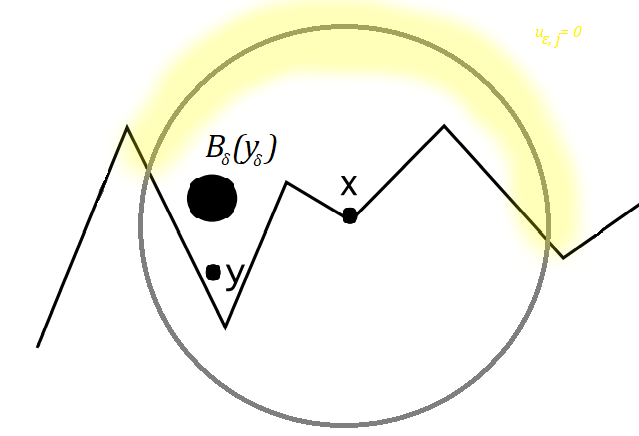
\includegraphics[scale = 0.5]{boundary.png}
	\end{center}
	Let $L := \on{Lip} (\gamma) + 2$ and set $y_\delta := y + \delta L e_d$, where $e_d \in \R^d$ is the $d$-th elementary basis vector and $\delta > 0$. It is clear that $B_\delta (y_\delta) \subseteq B_{r_j/2} (x_j)$ for $\delta \ll 1$. By Lipschitz continuity, for any $z \in B_\delta (y_\delta)$ we have
		\[ |\gamma(z') - \gamma(y')| < \on{Lip} (\gamma) |z' - y'| < \delta \on{Lip} (\gamma).  \]
	Then, since $z_d = y_d + \delta L +\delta \nu$ for some $|\nu| < 1$, we can write
		\[ \gamma(z') < \gamma(y') +\delta \on{Lip} (\gamma) < y_d +\delta \on{Lip} (\gamma) < z_d, \]
	i.e. $B_\delta (y_\delta) \subseteq \Omega \cap B_{r_j/2} (x_j)$, as desired. This implies that, given  $\phi_\delta \in C^\infty_c (|z| <\delta)$ a smooth approximation to the identity, the function
		\[ u_{\epsilon, j} (y) := \frac{1}{\delta^n} \int_{|z| < \delta} \phi_\delta (z) u  (y_\delta - z) \eta_j (y_\delta - z) \, dz\]
	is well-defined for $y \in \Omega \cap B_{r_j/2} (x_j)$ and satisfies $u_{\epsilon, j} \in C^\infty (\overline \Omega \cap B_{r_j/2} (x_j))$. Moreover, it vanishes in a neighborhood of $\Omega \cap \partial B_{r_j/2} (x_j)$ and thus can be extended by zero to view $u_{\epsilon, j} \in C^\infty (\overline \Omega)$. Choosing $\delta \ll 1$ and arguing as we did in the proof of smooth local approximation, 
		\[ || u_{\epsilon, j} - u \eta_j ||_{W^{k, p}} < \frac{\epsilon}{2N}. \]
	Setting $u_\epsilon = \sum_j u_{\epsilon, j}$, we conclude $u_\epsilon \in C^\infty (\overline \Omega)$ and, by the triangle inequality, 
		\[ ||u_\epsilon - u||_{W^{k, p}} \leq ||u_{\epsilon, 0} - u \eta_0||_{W^{k, p}} + \sum_{j  = 1}^N ||u_{\epsilon, j} - u \eta_j||_{W^{k, p}} < \epsilon . \]
\end{proof}

\begin{remark}
	The boundedness condition can be relaxed to the boundary condition that there exists a countable collection of $x_j \in \partial \Omega$ and radii $r_j > 0$ such that $\{ B_{r_j/2}(x_j) \}_j$ cover $\partial \Omega$ and the boundary is the graph of a Lipschitz function in $B_{r_j} (x_j)$. 
\end{remark}




\subsection{Duality}

For the positive Sobolev spaces, we see that differentiation lowers a function's regularity index, e.g. $\partial^\alpha u \in W^{k - |\alpha|, p} (\Omega)$ whenever $u \in W^{k,p} (\Omega)$. This  motivates the definition of Sobolev spaces with negative regularity; for $k \in \N$ and $1 \leq p \leq \infty$, we denote $W^{-k, p} (\Omega)$ the space of distributions $u \in C^\infty (\Omega)^*$ such that there exist $g_\alpha \in L^p (\Omega)$ satisfying
	\[ u = \sum_{|\alpha| \leq k} \partial^\alpha g_\alpha. \]
We equip this space with the norm
	\[ || u||_{W^{-k, p}} := \inf \left\{ \sum_{|\alpha| \leq k} ||g_\alpha||_{L^p} : g_\alpha \in L^p (\Omega) \text{ s.t. } u = \sum_{|\alpha| \leq k} g_\alpha \right\} .\]	
It is important to remark that $W^{-k, p} (\Omega)$ is not a space of \textit{functions}, but rather \textit{distributions}. 

\begin{theorem}[Dual of $W^{k, p}_0$]
	For $k \in \N_0$ and $1 < p < \infty$, each distribution $u \in W^{-k, p'} (\Omega)$ extends to a bounded linear functional on $W^{k, p}_0 (\Omega)$, and conversely every functional $u \in (W^{k, p}_0 (\Omega))^*$ admits a representation $u =  \sum_{|\alpha| \leq k} \partial^\alpha g_\alpha$ for $g_\alpha \in L^p (\Omega)$. 
That is, 
		\[ (W^{k, p}_0 (\Omega))^* \cong W^{-k, p'} (\Omega) \]
	as Banach spaces, with
		\[ ||u||_{(W^{k, p}_0 (\Omega))^*} = ||u||_{W^{-k, p'} (\Omega)}. \]	
\end{theorem}

\begin{proof}
	Let $u \in W^{-k, p'} (\Omega)$ and $g_\alpha \in L^{p'} (\Omega)$ such that $u = \sum_\alpha \partial_\alpha g_\alpha$, we claim that $u$ is a bounded functional with respect to the $W^{k, p}$-norm. Indeed, for $\phi \in C^\infty_c (\Omega)$, it follows by definition of the distributional derivative and Holder's inequality that	
		\[ \langle v, \phi \rangle = \sum_{|\alpha| \leq k} \langle \partial^\alpha g_\alpha, \phi \rangle = \sum_{|\alpha| \leq k} (-1)^{|\alpha|}  \langle g_\alpha, \partial^\alpha \phi \rangle \leq \sum_{|\alpha| \leq k} ||g_\alpha||_{L^{p'}} ||\partial^\alpha \phi||_{L^p} \leq ||\phi||_{W^{k, p}} \sum_{|\alpha| \leq k} ||g_\alpha||_{L^{p'}}.\]
	As $C^\infty_c (\Omega)$ is dense in $W^{k, p}_0 (\Omega)$, we can uniquely extend $v$ to a functional on	 $W^{k, p}_0 (\Omega)$. Optimizing in $g_\alpha$, it follows that $||u||_{(W^{k, p}_0)^*} \leq || u||_{W^{-k, p}}$ and thus $W^{-k, p'} (\Omega) \hookrightarrow (W^{k, p}_0 (\Omega))^*$.
		
	For the other inclusion, we argue by the Hahn-Banach theorem and Riesz representation. Let $\alpha_0, \dots, \alpha_K \in \N^d$ be an enumeration of multi-indices satisfying $|\alpha| \leq k$,  and define the operator $T: C^\infty_c (\Omega) \to L^p (\Omega)^K$ by 
		\[ Tv = (\partial^{\alpha_0} v, \dots, \partial^{\alpha_K} v). \]
	Endowing $C^\infty_c (\Omega)$ with the $W^{k, p}$-norm, it is clear that $T$ is injective and norm preserving. Thus for a functional $u \in (W^{k, p}_0 (\Omega))^*$, the functional $\widetilde u : T(C^\infty_c (\Omega)) \to \R$ given by 
		\[ \widetilde u(Tv) := u(v) \]
	is well-defined and bounded. By the Hahn-Banach theorem, $\widetilde u$ extends to a bounded linear function on $L^p (\Omega)^K$ with the same functional norm, so by the Riesz representation theorem there exist $\widetilde{g_{\alpha_0}}, \dots, \widetilde{g_{\alpha_K}} \in L^{p'} (\Omega)$ so that  
		\[ u(v) = \widetilde u (Tv) = \sum_{k = 0}^K \langle \widetilde{g_{\alpha_k}}, \partial^{\alpha_k} v \rangle = \sum_{k = 0}^K \langle \partial^{\alpha_k} g_{\alpha_k}, v \rangle  \]
	where $g_{\alpha_k} := (-1)^{|\alpha_k|} \widetilde{g_{\alpha_k}}$, and 
		\[ ||u||_{W^{-k, p}} \leq \sum_{k = 0}^K ||g_{\alpha_k}||_{L^p} \leq \sup_{v \in C^\infty_c (\Omega) \, : \, ||v||_{W^{k, p}} \leq 1} |u (v)| \leq ||u||_{(W^{k, p}_0 (\Omega))^*}, \]
	so we conclude 	$(W^{k, p}_0 (\Omega))^* \hookrightarrow W^{-k, p'} (\Omega)$. 
\end{proof}

\section{Extensions}	

Given a $C^k$-function on the upper half-space $\R^d_+$ with derivatives extending continuously to the boundary, Borel's lemma allows us to extend to a $C^k$-function on $\R^d$. Seeley's extension theorem \cite{Seeley64} provides a strengthening of this result, furnishing a linear map $E: C^k (\R^d_+) \to C^k (\R^d)$ which is continuous with respect to uniform convergence on compact sets. Following Seeley's reflection argument, we can prove an analogous extension theorem for Sobolev spaces. 

\begin{theorem}[Sobolev extension]
	Let $\Omega \subseteq \R^d$ be a bounded domain with $C^k$-boundary and $1 \leq p < \infty$. For each domain $V \subseteq \R^d$ such that $\overline \Omega \subseteq V$, there exists a bounded linear map $E: W^{k, p} (\Omega) \to W^{k, p} (\R^d)$ such that 
		\[ (Eu)_{|\Omega} = u, \qquad \supp Eu \subseteq V. \]	
\end{theorem}

\begin{proof}
	It suffices to define $E$ on the dense subspace $C^\infty (\overline \Omega) \subseteq W^{k, p} (\Omega)$. Denote $B \subseteq \R^d$ the ball of radius 1 centered at the origin. We reduce the problem to local extension by a partition of unity; since the boundary is $C^k$, for each $x \in \partial \Omega$ there exists an open neighborhood $x \in O_x$ and a $C^k$ diffeomorphism $\Psi_x : O_x \to B$ such that 
		\[ \Psi_x (O_x \cap \Omega)  = B \cap \R^d_+, \qquad \Psi_x (O_x \cap \partial\Omega)  = B \cap \partial\R^d_+. \]
	Choosing a smaller neighborhood if necessary, we can further assume $\overline{O_x} \subseteq V$. By compactness there exists a finite collection $O_1, \dots, O_N$ of such neighborhoods covering $\partial \Omega$. 	Let $O_0$ be an open set satisfying
		\[ \Omega \setminus \bigcup_{j = 1}^N O_j \subseteq O_0 \subseteq \overline{O_0} \subseteq \Omega.  \]
	Then $\{O_j\}_j$ furnishes an open covering of $\overline \Omega$, from which we construct $\{ \eta_j \}_j \subseteq C^\infty_c (\R^d)$ a smooth partition of unity subordinate to this covering. By construction $\eta_0 u$ extends by zero to view $\eta_0 u \in C^\infty (\R^d)$. For the boundary, terms, we claim that there exists a bounded extension map $\widetilde E: W^{k, p} (B \cap \R^d_+) \to W^{k, p} (B)$ such that
	\begin{itemize}
		\item if $\supp v \subseteq B \cap \overline{\R^d_+}$ then $\supp Ev \subseteq B$, 
		\item if $v \in C^k (B \cap \R^d_+)$ then $Ev \in C^k (B)$. 
	\end{itemize}
	In view of the first property, $\widetilde E((\eta_j u) \circ \Psi_j^{-1}) \circ \Psi_j \in C^k (O_j)$ and vanishes near $\partial O_j$, so it extends by zero to $\R^d$. We define the extension map $E$ by 
		\[ E u := \eta_0 u + \sum_{j = 1}^N \widetilde E((\eta_j u) \circ \Psi_j^{-1}) \circ \Psi_j. \]
	To establish the claim, we argue by a $k$-th order reflection procedure. Let $v \in C^k (B \cap \R^d_+)$ and define
		\[
			\widetilde E v (x)
				=
				\begin{cases}
					v(x) , 				&\text{if } x_d \geq 0, \\
					\sum_{i = 0}^k \alpha_i v (x', - \beta_i x_d) , 						&\text{if } x_d < 0,
				\end{cases}
		\]
	for some parameters $\alpha_i \in \R$ and $\beta_i > 0$. We aim to choose appropriate parameters such that $\widetilde E v \in C^k (B)$. To show that the derivatives up to order $k$ are continuous, we need to show that 
		\[ \lim_{z \downarrow 0} \partial^l_d (\widetilde E v)(x', z) = \lim_{z \uparrow 0} (\partial^l_d \widetilde E v)(x', z)   \]
	for $l = 0, 1, \dots, k$.	Note that 
		\[ \lim_{z \uparrow 0} \partial^l_d (\widetilde E v) (x', z) = \sum_{i = 0}^k \alpha_i (-\beta_i)^l \lim_{z \downarrow 0}  (\widetilde E v)(x', z).   \]
	Thus, it suffices to find $\alpha_i \in \R$ and $\beta_i > 0$ satisfying the compatability condition
	\[
		\begin{pmatrix}
			1 \\
			1\\
			\vdots \\
			1
		\end{pmatrix}
		=
		\begin{pmatrix}
			(-\beta_0)^0 & (-\beta_1)^0 &\dots & (-\beta_k)^0 \\
			(-\beta_0)^1 &  (-\beta_1)^1 & \dots & (-\beta_k)^1 \\
			\vdots 			& \vdots  & \ddots & \vdots \\
			(-\beta_0)^k &  (-\beta_1)^k &\dots & (-\beta_k)^k
		\end{pmatrix}
		\begin{pmatrix}
			\alpha_0 \\
			\alpha_1\\
			\vdots \\
			\alpha_k
		\end{pmatrix}.
	\]	
	The $(k + 1) \times (k + 1)$ matrix is a Vandermonde matrix, which is invertible for $\beta_i$ pairwise distinct, and thereby a choice of $\alpha_i$ exists such that the compatability condition holds, as desired. Note also that $\supp \widetilde E v \subseteq B$ whenever $\supp v \subseteq B \cap \overline{\R^d_+}$ and $\beta_k < 1$. It is clear from the chain rule that 
		\[ ||\widetilde E u||_{W^{k, p} (B)} \lesssim_{\alpha, \beta, k} ||u||_{W^{k, p} (B \cap \R^d_+)}. \]
	This completes the proof of the claim and thereby the theorem. 	
\end{proof}

\begin{remark}
	Our construction of the extension map depends on $k$, and as a technical requirement the boundary needed to be $C^k$ in order to perform the $k$-th order reflection procedure. E. Stein showed that there exists a universal extension operator $E$ that works on all $W^{k, p} (\Omega)$ with the weaker assumption that the boundary is $C^1$; see \cite{Stein16}. 
\end{remark}

The extension theorem allows us to view the Sobolev space on domains $\Omega \subseteq \R^d$ as localisations of Sobolev functions on $\R^d$. In particular, the Sobolev space $W^{k, p} (\Omega)$ is the image of the restriction mapping 
	\begin{align*}
		R: W^{k, p} (\R^d) 
			&\to W^{k, p} (\Omega),\\
		u
			&\mapsto u_{|\Omega}.	
	\end{align*}
This map induces a Banach space isomorphism between $W^{k, p} (\Omega)$ and a quotient space $W^{k, p} (\R^d)/\ker (R$. It is clear that the kernel of the restriction is exactly 
	\[  W^{k, p} (\R^d \setminus \Omega) := \{ u \in W^{k, p} (\R^d) : \supp u \subseteq \R^d \setminus \Omega \}. \]

\begin{corollary}
	Let $\Omega \subseteq \R^d$ be a bounded domain with $C^k$-boundary and $1 \leq p < \infty$, then 
		\[ W^{k, p} (\Omega) \cong W^{k, p} (\R^d) / W^{k, p} (\R^d \setminus \Omega) \]
	as Banach spaces, and in particular
		\[ ||u||_{W^{k, p} (\Omega)} \sim \inf_{v \in W^{k, p} (\R^d) \, : \, v_{|\Omega} = u} ||v||_{W^{k, p} (\R^d)} = \inf_{w \in W^{k, p} (\R^d \setminus \Omega)} || Eu + w ||_{W^{k, p} (\R^d)} . \]	
\end{corollary}

\begin{proof}
	The isomorphism holds algebraically in view of the first isomorphism theorem for vector spaces. We need to show equivalence of the norms. The last two norms are equivalent since 
		\[ (Eu + w)_{|\Omega} = u, \qquad v = Eu + (v - Eu), \qquad \supp (v - Eu) \subseteq \R^d \setminus \Omega \] 
	for all $v \in W^{k, p} (\R^d)$ satisfying $v_{|\Omega} = u$ and $w \in W^{k, p} (\R^d \setminus \Omega)$. It remains to prove the first norm is equivalent to the latter two. By boundedness of the extension map, 
		\[ \inf_{w \in W^{k, p} (\R^d \setminus \Omega)} ||Eu + w||_{W^{k, p} (\R^d)} \leq ||Eu||_{W^{k, p} (\R^d)} \lesssim ||u||_{W^{k, p} (\Omega)} .\]
	Conversely, let $v \in W^{k, p} (\R^d)$ satisfy $v_{|\Omega} = u$, then 
		\[ ||u||_{W^{k, p} (\Omega)} = \sum_{|\alpha| \leq k} ||\partial^\alpha u||_{L^p (\Omega)} \leq  \sum_{|\alpha| \leq k} ||\partial^\alpha v||_{L^p (\R^d)} = ||v||_{W^{k, p} (\R^d)}.  \]
	Taking the infimum finishes the proof. 		
\end{proof}

\section{Traces}

In general, a Sobolev function is not equivalent a.e. to a continuous function, and a $C^1$-boundary of a domain has measure zero, so the boundary values cannot be defined pointwise. Nevertheless, we can define the boundary values of suitable Sobolev functions at the expense of a loss of regularity on the boundary. 

\begin{theorem}[Sobolev trace]
	Let $\Omega \subseteq \R^d$ be a bounded domain with $C^1$-boundary and $1 < p < \infty$. Then there exists a bounded linear \emph{trace} map $T: W^{1, p} (\Omega) \to L^p (\partial \Omega)$ such that 
		\[ u_{|\partial \Omega} = Tu \]
	for all $u \in C^\infty (\overline \Omega)$. Moreover, the kernel is exactly $\ker T = W_0^{1, p} (\Omega)$.  	 
\end{theorem}

\begin{proof}
	It suffices by density to define $T$ for $u \in C^\infty (\overline \Omega)$. Let $\{ \eta_j \}_j \subseteq C^\infty_c (\R^d)$ be the partition of unity  and $\Psi_j : O_j \to B$ the $C^1$-diffeomorphisms as in the proof of the extension theorem. For $j \neq 0$ we set $v_j := (\eta_j u) \circ \Psi_j^{-1}$. Observe that $v_j \in C^1 (B \cap \R^d_+)$ and vanishes on $\partial B$. Thus
		\begin{align*}
			\int_{|x'| < 1} |v_j|^p dx' =  \int_{B \cap \R^d_+} \partial_d (|v_j|^p) dx =  p \int_{B \cap \R^d_+} |v_j|^{p - 1} \partial_d v_j \on{sgn} v_j \, dx \lesssim_p \int_{B \cap \R^d_+} (|v_j|^p + |\nabla v_j|^p) \, dx,
		\end{align*}	
	where the first equality follows from the divergence theorem and the inequality follows from Young's inequality. It follows from the change of variables formula that
		\[ ||u||_{L^p (\partial \Omega)} \lesssim ||u||_{W^{1, p} (\Omega)}. \]
	This proves existence of the trace operator.
	
	It is clear from definition that $W^{1, p}_0 (\Omega) \subseteq \ker T$; we omit the proof of the (much harder) converse. 
\end{proof}

\begin{remark}
	Regularity is necessarily lost for boundedness of the trace operator. Consider in one dimension the smooth maps $\phi_\epsilon : (0, 1) \to \R$ defined by 
	\[ \phi_\epsilon (x) = e^{-x^2/\epsilon} , \]
observe that $||\phi_\epsilon||_{L^1} \to 0$ as $\epsilon \to 0$, however $\phi_\epsilon (0) = 1$. 
\end{remark}

\begin{theorem}[Sobolev trace extension]
	Let $\Omega \subseteq \R^d$ be a bounded domain with $C^1$-boundary and $1 < p < \infty$. Then there exists a bounded linear trace extension map $S: W^{1 - 1/p, p} (\partial\Omega) \to W^{1,p} (\Omega)$ such that $TS = I$. 
\end{theorem}

\section{Sobolev embedding inequalities}

The Sobolev embedding inequalities trade regularity for integrability. As an illustration, consider $d = 1$, we claim that $W^{1, 1} (\R)$ continuously embeds into $C_0 (\R)$, paying an $L^1$-weak derivative to obtain continuity. Let $u \in C^\infty_c (\R)$, by the fundamental theorem of calculus, we can write
	\[ |u(x)| \leq \int_{-\infty}^x |u' (t)| dt \leq ||u'||_{L^1} \leq ||u||_{W^{1, 1}}. \]
The claim follows by density. 

\subsection{$L^p$-embedding inequalities}

To prove higher dimensional analogues, we follow the argument due to Gagliardo-Nirenberg via an isoperimetric-type inequality;
	

\begin{lemma}[Loomis-Whitney inequality]
	Let $d \geq 2$ and $f_j \in L^1 (\R^{d - 1})$ be measurable functions in the variables $x_1, \dots, x_{j - 1}, x_{j + 1}, \dots, x_d$ respectively, then 
		\[ \left|\left| \prod_{j = 1}^d f_j \right|\right|_{L^1 (\R^d)} \leq \prod_{j = 1}^d ||f_j||_{L^{d - 1} (\R^{d - 1})} \]
\end{lemma}

\begin{proof}
	We integrate with respect to $x_1$, noting $f_1$ is independent of $x_1$, and apply Holder's inequality,
		\[ \int_{\R} \left|\prod_{j  =1 }^d f_j\right| dx_1 \leq f_1 \prod_{j = 2}^d ||f_j||_{L^{d - 1}_{x_1}}. \]
	Integrating with respect to $x_2$, noting $||f_2||_{L^{d - 1}_{x_2}}$ is independent of $x_2$, and applying Holder's inequality, 
		\[ \int_{\R} \left|\prod_{j  =1 }^d f_j \right| dx_1 dx_2 \leq ||f_1||_{L^{d - 1}_{x_2}} ||f_2||_{L^{d - 1}_{x_1}} \prod_{j = 3}^d ||f_j||_{L^{d - 1}_{x_1, x_2}} .\]
	Iterating this procedure, we obtain the desired inequality. 
\end{proof}

\begin{remark}
	Geometrically, the Loomis-Whitney inequality controls the size of a set by the product of the size of its projections to the coordinate hyperplanes. Let $\pi_j : \R^d \to \R^{d - 1}$ be $(x_1, \dots, x_d) \mapsto (x_1, \dots, x_{j - 1}, x_{j + 1}, \dots, x_d)$, then, for any measurable set $E \subseteq \R^d$, taking $f_j = \mathbb 1_{\pi_j (E)}$ in the Loomis-Whitney inequality furnishes
		\[ |E| = \left| \left| \prod_{j = 1}^d \mathbb 1_{\pi_j (E)} \right| \right|_{L^1 (\R^d)}  \leq \prod_{j = 1}^d ||\mathbb 1_{\pi_j (E)} ||_{L^{d - 1} (\R^{d - 1})} = \prod_{j = 1}^d |\pi_j (E)|^{\frac{1}{d - 1}}. \]
\end{remark}

\begin{theorem}[Homogeneous Sobolev inequality]
	For $d \geq 2$ and $k \in \N$, suppose that $u \in C^\infty_c (\R^d)$, then 
		\[ ||u||_{L^q} \lesssim ||\nabla^k u||_{L^p} \]
	for $1 \leq p < q < \infty$ satisfying $\tfrac{1}{p} - \tfrac{1}{q}	= \tfrac{k}{d}$. Moreover, given a domain $\Omega \subseteq \R^d$, we have $W^{k, p}_0 (\Omega) \subseteq L^q (\Omega)$ and, if it is bounded with $C^k$-boundary, $W^{k, p} (\Omega) \subseteq L^q (\Omega)$. 
\end{theorem}

\begin{proof}
	Applying the inequality inductively, it suffices to prove the result for $k = 1$. Consider first the case $p = 1$; by the fundamental theorem of calculus, as well as the assumption that $u$ is compactly supported, for $j = 1, \dots, d$ we can write
		\[ |u(x)| \leq \int_{-\infty}^{x_j} |\partial_j u(x_1, \dots, te_j, \dots, x_d)| dt \leq \int_{\R} |\nabla u (x)| dx_j.\]
	It follows that
		\[ |u(x)|^{\frac{d}{d - 1}} \leq \prod_{j = 1}^d \left( \int_{\R} |\nabla u (x)| dx_j \right)^{\frac{1}{d - 1}}. \]
	Integrating and applying the Loomis-Whitney inequality to the product on the right, we obtain
		\begin{align*}
			 \int_{\R^d} |u(x)|^{\frac{d}{d - 1}} dx 
			 	&\leq \int_{\R^d}  \prod_{j = 1}^d \left(  \int_{\R} |\nabla u (x)| dx_j \right)^{\frac{1}{d - 1}} dx \leq \prod_{j = 1}^d \left|\left| \left( \int_{\R} |\nabla u (x)| dx_j \right)^{\frac{1}{d - 1}}\right|\right|_{L^{d - 1} (\R^{d - 1})} = ||\nabla u||_{L^1}^{\frac{d}{d - 1}}.
		\end{align*}	 	
	Rearranging furnishes the inequality. Suppose now $1 < p < d$, then applying the $p = 1$ case to $|u|^q$, it follows by the chain rule and Holder's inequality that 
	\begin{align*}
		\int_{\R^d} |u|^q dx 
			&\leq \left( \int_{\R^d} \nabla (|u|^{\frac{d - 1}{d}q})dx \right)^{\frac{d}{d - 1}} \sim_{d, q} \left( \int_{\R^d} |\nabla u| |u|^{\frac{d - 1}{d}q - 1}dx \right)^{\frac{d}{d - 1}}  \leq \left( || |u|^{ \frac{d - 1}{d} q - 1}||_{L^{\frac{p}{p - 1}}} ||\nabla u||_{L^p}\right)^{\frac{d}{d - 1}}.
	\end{align*}
	Note that 
		\[ \frac{p}{p - 1} \left(\frac{d - 1}{d} q - 1 \right) = q, \qquad \frac{d}{d - 1} \left(\frac{d - 1}{d} q - 1 \right) = q - \frac{d}{d - 1}.\]
	Rearranging factors, the desired inequality follows. Let $\Omega \subseteq \R^d$ be a domain, the inequality extends by density for $u \in W^{1,p}_0 (\Omega)$ and thus $W^{1, p}_0 (\Omega) \subseteq L^q (\Omega)$. If $\Omega$ has a $C^1$-boundary, it follows from the extension theorem that
		\[ ||u||_{L^q (\Omega)} \leq ||u||_{L^q (\R^d)} \lesssim || u||_{W^{1 ,p} (\R^d)} \lesssim ||u||_{W^{1, p} (\Omega)} \]
	for $u \in W^{1, p} (\Omega)$, and hence $W^{1, p} (\Omega) \subseteq L^q (\Omega)$.
\end{proof}

\begin{remark}
	The endpoint case $(p, q) = (d, \infty)$ fails when $d \geq 2$. For instance, the function 
		\[ u(x) = \log \log \left(1 + \frac{1}{|x|} \right) \]
	is contained in $W^{1, d} (|x| < 1)$, however it is unbounded near $x = 0$. By applying a smooth cut-off and mollifying, we can also produce a family of counter-examples on $\R^d$. 
\end{remark}

\begin{theorem}[Inhomogeneous Sobolev inequality]
	For $d \geq 2$ and $k \in \N$, suppose that $u \in C^\infty_c (\R^d)$, then 
		\[ ||u||_{L^q} \leq || u||_{W^{k, p}} \]
	for $1 \leq p < q < \infty$ satisfying $\tfrac{1}{p} - \tfrac{1}{q} \leq \tfrac{k}{d}$. Moreover, given a domain $\Omega \subseteq \R^d$, we have $W^{k, p}_0 (\Omega) \subseteq L^q (\Omega)$ and, if it is bounded with $C^1$-boundary, $W^{k, p} (\Omega) \subseteq L^q (\Omega)$. 
\end{theorem}

\begin{proof}
	Assume without loss of generality $k$ is the smallest integer such that $\tfrac{1}{p} - \tfrac{1}{q} \leq \tfrac{k}{d}$. Choose $1 \leq p < q < r < \infty$ satisfying $\tfrac{1}{p} - \tfrac{1}{r} = \tfrac{k}{d}$, then interpolating norms and applying the homogeneous Sobolev embedding
		\[ ||u||_{L^q} \leq ||u||^\theta_{L^p} ||u||^{1 - \theta}_{L^r} \lesssim ||u||^\theta_{L^p} ||\nabla^k u||_{L^p}^{1 - \theta} \lesssim ||u||_{W^{k, p}}, \]
	as desired. 	
\end{proof}

\begin{remark}
	As a general heuristic, higher regularities always control lower regularities, and lower exponents always control higher exponents (Littlewood's principle: ``larger exponents are always on the left''). One can verify that the numerology for the exponents in the homogeneous Sobolev embedding is necessary via dimensional analysis. 
\end{remark}

\subsection{$C^{0, \gamma}$-embedding inequalities}

\textit{A priori} a Sobolev function is defined pointwise only up to a.e. modification. However, provided sufficient regularity, the Sobolev space embeds into a space of continuous functions, allowing for a canonical and continuous choice of pointwise values. We rely on a potential estimate:

\begin{lemma}
	Let $u \in C^1 (\overline{B_R (x)})$ for some $R> 0$ and $x \in \R^d$, then 
		\[ \frac{1}{|B_R (x)|} \int_{B_R (x)} |u(y) - u(x)| dy \lesssim_d \int_{B_R (x)} \frac{|\nabla u (y)|}{|x - y|^{d - 1}} dy, \]
	and if $u \in C^1_c (\R^d)$, then 
		\[ |u(x)| \leq \int_{\R^d} \frac{|\nabla u (y)|}{|x - y|^{d - 1}} dy. \]	
\end{lemma}

\begin{proof}
	We can write
		\[  \int_{B_R (x)} |u(y) - u(x)| dy  = \int_0^R \int_{|x - y| = r} |u(y) - u(x)| dS(y) d r. \]
	By the fundamental theorem of calculus and a change of variables between polar and rectangular coordinates, we can estimate the integral on $|x - y| = r$ as
		\begin{align*}
			 \int_{|x - y| = r} |u(y) - u(x)| dS(y) 
			 	&= r^{d - 1} \int_{|z| = 1} |u(x + rz) - u(x)| dS(z) \\
			 	&\leq r^{d - 1} \int_{|z| = 1} \int_0^r |\nabla u (x + tz) | dt dS(z) = r^{d - 1} \int_{|x - y| \leq r} \frac{|\nabla u(y)|}{|x - y|^{d - 1}} dy. 		 	
		\end{align*}	
	Since $r^{d - 1}$ is comparable to the surface area of $|x - y| = r$, taking $r \to \infty$ gives the result for $u \in C^1_c (\R^d)$. If we instead integrated with respect to $r$, we obtain
		\[ \int_0^R \int_{|x - y| = r} |u(y) - u(x)| dS(y) d r \leq \int_0^R r^{d - 1} \int_{|x - y| \leq r} \frac{|\nabla u(y)|}{|x - y|^{d - 1}} dy dr\leq \frac1d R^d \int_{B_R (x)} \frac{|\nabla u(y)|}{|x - y|^{d - 1}} dy. \]	
	Since $R^d$ is comparable to the volume of $B_R (x)$, rearranging furnishes the result. 	
\end{proof}

\begin{theorem}[Homogeneous Morrey's inequality]
	For $k,r \in\N$, suppose that $u \in C^\infty_c (\R^d)$, then 
		\[ [\nabla^r u]_{C^{0, \gamma}} \lesssim || \nabla^k u||_{L^p}, \qquad  ||u||_{C^{r, \gamma}} \lesssim ||u||_{W^{k, p}} \]
	for $1 < p < \infty$ and $0 < \gamma < 1$ satisfying $\gamma = k - r - \tfrac{d}{p}$. Moreover, given a domain $\Omega \subseteq \R^d$, we have $W^{1, p}_0 (\Omega) \subseteq C^{0, \gamma} (\Omega)$ and, if it is bounded with $C^1$-boundary, $W^{1, p} (\Omega) \subseteq C^{0, \gamma} (\Omega)$.
\end{theorem}

\begin{proof}
	It suffices to prove the result for $k = 1$ and $r = 0$, as combined with the homogeneous Sobolev inequality 
		\[ [\nabla^r u]_{C^{0, \gamma}} \lesssim ||\nabla^{r + 1} u||_{L^q} \lesssim ||\nabla^k u||_{L^p} \]
	for $1 < q < \infty$ satisfying $\tfrac{1}{p} - \tfrac{1}{q}= \tfrac{k - r - 1}{d}$. Applying the $k = 1$ and $r = 0$ case inductively gives control over the $C^r$-norm. We begin then by controlling the $L^\infty$-norm of $u$; let $R > 0$ and $x \in \R^d$, then by the triangle inequality, the previous lemma, and Holder's inequality
		\begin{align*}
			 |u(x)|
			 	&\leq \frac{1}{|B_R (x)|} \int_{B_R (x)} |u(x) - u(y)| dy + \frac{1}{|B_R (x)|} \int_{B_R (x)} |u(y)| dy .
		\end{align*}	 	
	The second term on the right is controlled by Holder's inequality,
		\[ \frac{1}{|B_R (x)|} \int_{B_R (x)} |u(y)| dy \lesssim R^{- \frac{d}{p}} ||u||_{L^p (\R^d)} .\]	
	The first term on the right is controlled by the previous lemma and Holder's inequality, 
		\begin{align*}
			\frac{1}{|B_R (x)|} \int_{B_R (x)} |u(x) - u(y)| dy \lesssim \int_{B_R (x)} \frac{|\nabla u (y)|}{|x - y|^{d  - 1}} dy \lesssim || |x - y|^{1 - d} ||_{L^{p'}_y (B_R (x))} ||\nabla u||_{L^p (\R^d)} \sim R^\alpha ||\nabla u||_{L^p (\R^d)}.
		\end{align*}
	Taking $R = 1$, we obtain 
		\[ ||u||_{L^\infty} \lesssim ||u||_{W^{1, p}}.  \]
	Next, we estimate the Holder semi-norm; for $|x - y| = R$, we have
		\begin{align*}
			 |u(x) -u(y)| 
			 	&\leq \frac{1}{|B_R (x) \cap B_R (y)|} \int_{B_R (x) \cap B_R (y)} \left( |u(x) - u(z)| + |u(z) - u(y)| \right) dz \\
			 	&\lesssim \frac{1}{|B_R (x)|} \int_{B_R (x)} |u(x) - u(z)| dz + \frac{1}{|B_R (y)|} \int_{B_R (x)} |u(y) - u(z)| dz \\
			 	&\lesssim \int_{B_R (x)} \frac{|\nabla u(z)|}{|x - z|^{d - 1}} dz + \int_{B_R (y)} \frac{|\nabla u(z)|}{|y - z|^{d - 1}} dz \lesssim R^\gamma ||\nabla u||_{L^p (\R^d)}
		\end{align*}	 	
	where the first inequality follows from the triangle inequality, the second holds since the volumes of $B_R (x)$ and $B_R(y)$ are comparable to their intersection $B_R (x) \cap B_R (y)$, the third from the previous lemma, the fourth from Holder's inequality. Rearranging and optimising in $|x - y| = R$, we obtain
		\[ [u]_{C^{0, \gamma}} \lesssim ||\nabla u||_{L^p} \leq ||u||_{W^{1, p}}, \]
	proving the inequality. Let $\Omega \subseteq \R^d$ be a domain, the inequality extends by density for $u \in W^{1, p} (\Omega)$ and thus $W^{1, p}_0 (\Omega) \subseteq C^{0, \gamma} (\Omega)$. If $\Omega$ is also bounded and $C^1$, it follows from the extension theorem that
		\[ ||u||_{C^{0, \gamma} (\Omega)} \leq ||u||_{C^{0, \gamma} (\R^d)} \lesssim ||u||_{W^{1, p} (\R^d)} \lesssim ||u||_{W^{1,p} (\Omega)} \]
	for $u \in W^{1, p} (\Omega)$, and hence $W^{1, p} (\Omega) \subseteq C^{0, \gamma} (\Omega)$. 	
\end{proof}

\begin{theorem}[Inhomogeneous Morrey's inequality]
	For $k, r \in \N$, suppose that $u \in C^\infty_c (\R^d)$, then 
		\[ ||u||_{C^{r, \gamma}} \lesssim ||u||_{W^{k, p}} \]
	for $1 < p < \infty$ and $0 < \gamma < 1$ satisfying $\gamma \leq k - r - \tfrac{d}{p}$. Moreover, given a domain $\Omega \subseteq \R^d$, we have $W^{1, p}_0 (\Omega) \subseteq C^{0, \gamma} (\Omega)$ and, if it is bounded with $C^1$-boundary, $W^{1, p} (\Omega) \subseteq C^{0, \gamma} (\Omega)$.
\end{theorem}

\begin{proof}
	Assume without loss of generality $k$ is the smallest integer satisfying $\gamma \leq k - r - \tfrac{d}{p}$. Choose $0 < \gamma \leq \alpha < 1$ satisfying $\alpha = k - r - \tfrac{d}{p}$, then it follows from the homogeneous Morrey's inequality that
		\[ ||u||_{C^{r, \gamma}} \leq ||u||_{C^{r, \alpha}} \lesssim ||u||_{W^{k, p}}, \]
	as desired. 	
\end{proof}


\section{Compact embedding}

Given a bounded sequence in either a Sobolev or Holder space, we have uniform control over a higher order term which guarantees \textit{equicontinuity}. It follows from compactness lemmas that we can pass to a subsequence converging in a lower regularity space. In summary, regularity can be traded to upgrade Sobolev embedding to a compact embedding. 

\begin{lemma}[Arzela-Ascoli]
	Let $K \subseteq \R^d$ be compact. A family of continuous functions $\cF \subseteq C(K)$ is pre-compact if and only if it satisfies
	\begin{itemize}
		\item \emph{uniform boundedness}; $||u||_{L^\infty} \lesssim 1$ uniformly in $u \in \cF$, 
		\item \emph{equicontinuity}; for every $\epsilon > 0$ there exists $\delta > 0$ such that 
					\[ |u (x) - u (y)| < \epsilon \qquad \text{whenever } |x - y| < \delta \]
				for all $x, y \in K$ and $u \in \cF$. 	
	\end{itemize}
\end{lemma}

\begin{remark}
	Uniform boundedness can be weakened to pointwise boundedness, that is, the condition that $|f(x)| \lesssim_x 1$ uniformly in $f \in \cF$. This is because equicontinuity and compactness of $K$ allow us to guarantee pointwise boundedness to uniform boundedness. 
\end{remark}


\begin{theorem}[Compactness of Holder spaces]
	Let $K \subseteq \R^d$ be compact and $0 < \alpha \leq \beta \leq 1$, then 
		\[ C^{0, \beta} (K) \Subset C^{0, \alpha} (K). \]
	Moreover, if $\Omega \subseteq \R^d$ is a bounded $C^1$-domain, then 
		\[ W^{1, p} (\Omega) \Subset C^{0, \alpha} (\Omega), \]
	for $d < p \leq \infty$ and $0 < \alpha < 1 - \tfrac{d}{p}$.
\end{theorem}

\begin{proof}
	Recall that complex-valued uniformly continuous functions extend continuously to the closure of their domains, so $C^{0, \alpha} (\Omega) = C^{0, \alpha} (\overline \Omega)$, so this reduces the case of bounded domains to compact domains. It is clear that
		\[ [u]_{C^\alpha} \leq \diam (K)^{\beta - \alpha} [u]_{C^\beta},\]
	so $C^{0, \beta} (	K)$ embeds continuously into $C^{\alpha} (K)$. Moreover, this embedding is compact; let $\{ u_k \}_k \subseteq C^{0, \beta} (K)$ be bounded, then the sequence is uniformly bounded with respect to the $L^\infty$-norm and equicontinuous, 
		\[ ||u_k||_{L^\infty} \leq ||u_k||_{C^{0, \beta}} \lesssim 1, \qquad |u_k (x) - u_k (y)| \leq [u_k]_{C^\beta} |x - y|^\alpha \lesssim |x - y|^\alpha. \]
	It follows from Arzela-Ascoli that we can pass to a subsequence such that $||u_k - u||_{L^\infty} \to 0$ for some $u \in C(K)$. It remains to show that $[u_k - u]_{C^\alpha} \to 0$; indeed, denoting $v_k = u_k - u$, we can write
		\begin{align*}
			[v_k]_{C^\alpha} 
				&= \sup_{x \neq y} \frac{|v_k (x) - v_k (y)|}{|x - y|^\alpha} =  \sup_{x \neq y} \left( \frac{|v_k (x) - v_k (y)|}{|x - y|^\beta}\right)^{\frac\alpha\beta} |v_k (x) - v_k (y)|^{1 - \frac\alpha\beta} \\
				&\leq [v_k]_{C^\beta}^{\frac\alpha\beta} 2^{1 - \frac\alpha\beta} ||v_k||_{L^\infty}^{1 - \frac\alpha \beta} \lesssim_{\alpha, \beta} ||v_k||_{L^\infty}^{1 - \frac\alpha \beta} \overset{k \to \infty}{\longrightarrow} 0.
		\end{align*} 		
	This completes the proof. 	
\end{proof}

\begin{lemma}[Frechet-Kolmogorov]
	For $1 \leq p < \infty$, a family $\cF \subseteq L^p (\R^d)$ is pre-compact if and only if it satisfies
	\begin{itemize}
		\item \emph{uniform boundedness}; $||u||_{L^p} \lesssim 1$ uniformly in $u \in \cF$, 
		\item \emph{equicontinuity}; for every $\epsilon > 0$ there exists $\delta > 0$ such that 
					\[ ||u(x) - u(x - h)||_{L^p_x} < \epsilon\]
				for all $|h| < \delta$ and $u \in \cF$, 
		\item \emph{tightness}; for all $\epsilon > 0$ there exists $R> 0$ such that 
					\[ ||u||_{L^p (|x| > R)} < \epsilon \]
				for all $u \in \cF$. 	
	\end{itemize}
\end{lemma}

\begin{theorem}[Rellich-Kondrachov compactness]
	Let $\Omega \subseteq \R^d$ be a bounded $C^1$-domain and let $1 \leq p < d$, then 
		\[ W^{1, p} (\Omega) \Subset L^r (\Omega) \]
	for $1 \leq r < q$ where $q$ is the Sobolev conjugate, i.e. $\tfrac1p - \tfrac1q = \tfrac1d$
\end{theorem}

\begin{proof}
	We argue by Frechet-Kolmogorov, i.e. we want to show the unit ball in $W^{1, p} (\Omega)$ is bounded, equicontinuous, and tight in $L^r (\Omega)$. Recall that $L^q (\Omega)$ continuously embeds into $L^r (\Omega)$, with implicit constant depending on the measure of $\Omega$, so, combining with Sobolev embedding, we know $W^{1, p} (\Omega)$ embeds continuously into $L^r (\Omega)$,
		\[ ||u||_{L^r} \lesssim_\Omega ||u||_{L^q} \lesssim ||u||_{W^{1, p}}. \]
	In particular, the unit ball in $W^{1, p} (\Omega)$ is also bounded in $L^r (\Omega)$. Tightness is trivial since the domain $\Omega$ is bounded, so it remains to show $L^r$-equicontinuity. We argue by interpolating, controlling the $L^r$-norm by the $L^1$ and $L^q$-norms. Let $u \in W^{1, p} (\Omega)$ be smooth, then by the fundamental theorem of calculus 
		\[ u(x) - u(x - h) = \int_0^1 h \cdot \nabla u(x - th) dt. \]
	Taking the $L^1$-norm and applying Cauchy-Schwarz and Fubini's theorem gives	
		\[ ||u(x) - u(x - h)||_{L^1_x}  \leq |h| \, ||\nabla u||_{L^1} \lesssim_\Omega |h| \, ||\nabla u||_{L^p} \leq |h| \, ||u||_{W^{1, p}}. \]
	It follows from density that this estimate holds for all $u \in W^{1, p} (\Omega)$. By the triangle inequality and Sobolev embedding, 
		\[ ||u(x) - u(x - h)||_{L^q_x} \leq 2 ||u||_{L^q} \lesssim ||u||_{W^{1, p}}.\]	
	Let $0 < \theta < 1$ satisfy $\tfrac1r = \tfrac\theta1 + \tfrac{1 - \theta}{q}$, then collecting the inequalities above and interpolating we obtain
		\begin{align*}
			 ||u(x) - u(x - h)||_{L^r_x}
			 	&\leq ||u(x) - u(x - h)||_{L^1_x}^\theta ||u(x) - u(x - h)||_{L^q_x}^{1 - \theta} \lesssim |h|^\theta ||u||_{W^{1, p}}. 
		\end{align*}	 
	This proves that the unit ball in $W^{1, p} (\Omega)$ is equicontinuous, completing the proof.
\end{proof}

\begin{remark}
	We also have
		\[ W^{1, p} (\Omega) \Subset L^p (\Omega) \]
	for every $1 \leq p \leq \infty$. The case $1 \leq p < d$ follows from Rellich-Kondrachov since the Sobolev conjugate obeys $p < q$. The case $d < p \leq \infty$ follows from Morrey's inequality and compactness of Holder spaces. 	
\end{remark}

\begin{corollary}[Poincare inequality]
	Let $\Omega \subseteq \R^d$ be a bounded $C^1$-domain, then 
		\[ \left|\left| u - \frac{1}{|\Omega|} \int_\Omega u(y) dy \right|\right|_{L^p} \lesssim ||\nabla u||_{L^p} \]
	for all $1 \leq p \leq \infty$ and $u \in W^{1, p} (\Omega)$. In particular, $||u||_{W^{1, p}} \sim ||\nabla u||_{L^p}$ for $u$ with mean zero. 
\end{corollary}

\begin{proof}
	It suffices to prove the result for functions with mean zero; indeed we replace $u$ with
		\[ v:=  u - \frac{1}{|\Omega|} \int_\Omega u(y) dy, \]
	which has mean zero and $\nabla u = \nabla v$. We argue by contradiction, assuming that for all $n \in \N$ there exists $v_n \in W^{1, p} (\Omega)$ with mean zero satisfying 
		\[ ||v_n||_{L^p} \geq n ||\nabla v_n||_{L^p}. \]
	Normalizing the left-hand side, we can assume $||v_n||_{L^p} = 1$. It follows that $|| v_n||_{W^{1, p}} \leq 2$, so Rellich-Kondrachov allows us to pass to a subsequence such that $v_n \to v_\infty$ for some $v_\infty \in L^p (\Omega)$. On the other hand, $||\nabla v_n||_{L^p} \to 0$, so $\nabla v_\infty \equiv 0$ in the sense of distributions, i.e. $v_\infty$ is a.e. constant. Since $L^p$-convergence implies $L^1$-convergence in bounded domains, we have convergence of means,  
		\[ v_\infty =  \frac{1}{|\Omega|} \int_\Omega v_\infty (y) dy = \lim_{n \to \infty} \frac{1}{|\Omega|} \int_\Omega v_n (y) dy = 0.  \]
	However, $||v_\infty||_{L^p} = \lim_n ||v_n||_{L^p} = 1$, a contradiction. 
\end{proof}

\bibliography{biblio}
\bibliographystyle{alpha} 

\end{document}